\chapter[Sterowanie modelem robota z \emph{Small-size League}]{Sterowanie modelem robota z \emph{Small-size League} \label{chap:holonomic}}
%\chaptermark{holonomic}
Budowę i napęd robota należy dobrać odpowiednio do postawionego zadania. W przypadku ligi \emph{Small-size League}, najważniejszym elementem jest prostota i mobilność
takiej jednostki. W pracy inżynierskiej \cite{inzynierka} posługiwano się  modelem o napędzie różnicowym (dwa niezależnie napędzane koła). Decyzję o odwzorowaniu takiego robota
w symulatorze motywowano wtedy próbą odzwierciedlenia rzeczywistego robota \texttt{HMT} \cite{hamada_mgr} stworzonego w ramach koła robotyki \texttt{Bionik} działającego na Wydziale Elektroniki i Technik Informacyjnych Politechniki
Warszawskiej. W niniejszej pracy zrezygnowano jednak z tego modelu, ponieważ nie był wystarczająco funkcjonalny. Zdecydowano się natomiast na zbudowanie modelu wzorowanego na rzeczywistym zawodniku \emph{Small-size League}.  
\section{Omówienie omnikierunkowej bazy jezdnej}
Analogicznie jak podczas rzeczywistej rozgrywki, decydującym elementem jest budowa anatomiczna i zdolności motoryczne zawodników. Tak samo podczas
rozgrywek robotów istotna rolę odgrywa baza jezdna zawodników.  W zawodach wykorzystywana jest baza omnikierunkowa, ponieważ jest ona najłatwiejsza w użyciu. Korzystając z takiej bazy w
większości algorytmów robot może być traktowany jako punkt materialny.
\subsection{Opis położenia kół}
Baza omnikierunkowa składa się z umieszczonych symetrycznie co najmniej trzech kół szwedzkich (tak jak zaprezentowano to na rysunku \ref{fig:holonomic_base}).
Każde z kół posiada osobny napęd. Budowę koła omnikierunkowego przedstawiono na ilustracji \ref{fig:omnidirectional_wheel}. 
\begin{figure}[h!]
\centering
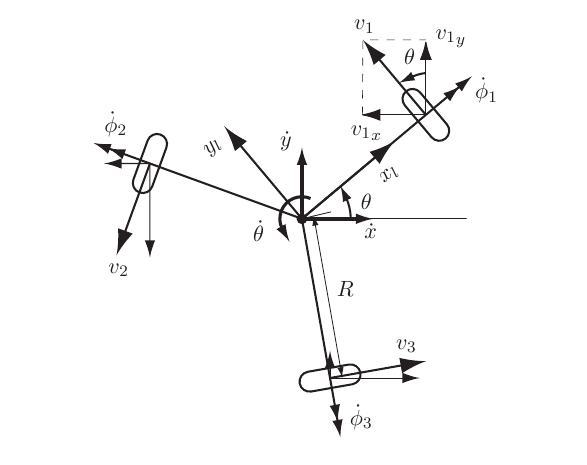
\includegraphics[scale=0.7]{./holonomic/holonomic_base}
\caption{ Rozkład kół w omnikierunkowej bazie jezdnej }\label{fig:holonomic_base}
\end{figure}
Koło szwedzkie posiada na swoim obwodzie zamontowane w odpowiedni sposób dodatkowe rolki. Umożliwiają one ruch koła w dowolnym kierunku, bez względu na to, 
jak koło jest zorientowane w przestrzeni. Dzięki temu taką bazę jezdną można zaliczyć klasy holonomicznych.
\begin{figure}[h]
\centering
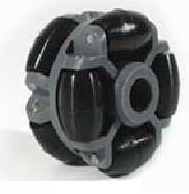
\includegraphics[scale=0.7]{./holonomic/omnidirectional_wheel}
\caption{ Konstrukcja przykładowego koła szwedzkiego }\label{fig:omnidirectional_wheel}
\end{figure}
\subsection{Opis kinematyki oraz dynamiki bazy}
Podczas sterowania robotem istotnym problemem jest sposób w jaki prędkości i przyspieszenia obrotowe poszczególnych kół przekładają się
na predkość/przyspieszenie kątowe i liniowe całego robota. Wszystkie poniższe obliczenia zostały wykonane przy założeniu, że koła nie ulegają poślizgowi.
Przy tym uproszczeniu cały moment obrotowy silników przekłada się na prędkość robota.
Przyspieszenie liniowe i prędkość obrotowa środka masy takiego układu dane jest następującymi wzorami:
\begin{equation}
a=\frac{1}{M}(F1+F2+F3)
\end{equation}

\begin{equation}
\dot{ \omega }=\frac{R}{I}(f_1+f_2+f_3)
\end{equation}
, gdzie $f_i$ oznacza długość wektora siły przyłożonego do poszczególnego koła, a $I$  jest momentem bezwładności.
Przyspieszenie wzdłuż poszczególnych osi można obliczyć rozbijając siłę działającą na koło wzdłuż tychże osi, otrzymamy wtedy:
\begin{equation}
Ma_x=-f_1sin\theta_1 - f_2sin\theta_2 - f_3sin\theta_3
\end{equation}
\begin{equation}
Ma_y=f_1cos\theta_1 + f_2cos\theta_2 + f_3cos\theta_3
\end{equation}
Dla jednolitego cylindra moment bezwładności obliczany jest ze wzoru $I=\frac{1}{2}MR^2$, natomiast dla obręczy $I=MR^2$, gdzie $R$ jest odpowiednio promieniem
\mbox{cylindra/obręczy} natomiast $M$ masą. Dla obiektów o rozkładzie masy pomiędzy
obręczą, a cylindrem wprowadzany jest dodatkowy parametr $\alpha$. Wzór przyjmuje wtedy postać: $I=\alpha MR^2$, gdzie $0<\alpha<1$.
Używając zapisu macierzowego równania można przedstawić w postaci:
\begin{equation}
 \begin{pmatrix}
  a_x\\
  a_y\\
  \dot{\omega}
 \end{pmatrix}
  =
\begin{pmatrix}
  -sin\theta_1 & -sin\theta_2 & -sin\theta_3 \\
  cos\theta_1 & cos\theta_2 & cos\theta_3 \\
  \frac{MR}{I} & \frac{MR}{I} & \frac{MR}{I}\\
 \end{pmatrix} 
 \begin{pmatrix}
  f_1\\
  f_2\\
  f_3
 \end{pmatrix}
\end{equation}

Podstawiając do powyższego wzoru $I=\alpha MR^2$ oraz zastępując $\dot{\omega}$ wyrażeniem $R\dot{\omega}$ otrzymujemy:
\begin{equation}
 \begin{pmatrix}
  a_x\\
  a_y\\
  R\dot{\omega}
 \end{pmatrix}
  =
\begin{pmatrix}
  -sin\theta_1 & -sin\theta_2 & -sin\theta_3 \\
  cos\theta_1 & cos\theta_2 & cos\theta_3 \\
  \frac{1}{\alpha} & \frac{1}{\alpha} & \frac{1}{\alpha}\\
 \end{pmatrix} 
 \begin{pmatrix}
  f_1\\
  f_2\\
  f_3
 \end{pmatrix}
\end{equation}

Macierz z powyższego równania o wymiarze $3x3$ zostanie oznaczona symbolem~$C_{\alpha}$.

Jednak najbardziej interesujący jest sposób w jaki prędkość obrotowa kół przekłada się na prędkość liniową robota.
Załóżmy, że robot porusza się wzdłuż osi OX, zatem wektor prędkości $(\upsilon_{x}, \upsilon_{y}, R\omega)$ wygląda następująco $(1,0,0)$.
Rozważmy jedno z kół, tak jak to przedstawiono na rysunku \ref{fig:linear_speed}. Dokonując rozkładu wektora prędkości na dwie składowe, jedną zgodną z ruchem
obrotowym dużego koła, a drugą zgodną z ruchem małych, poprzecznych kółek otrzymujemy odpowiednio prędkości $\upsilon=-sin\theta$ $\upsilon_{y}=cos\theta$.
Przy wyznaczaniu prędkości koła przyjęto założenie, że prędkość dodatnia powoduje obrót w kierunku wyznaczonym przez kciuk prawej dłoni, gdy pokrywa się ona z osią 
silnika.
Otrzymujemy zatem następujące powiązanie pomiędzy prędkościami robota a prędkościami poszczególnych silników:
 \begin{equation}
 \begin{pmatrix}
  \upsilon_1\\
  \upsilon_2\\
  \upsilon_3
 \end{pmatrix}
  =
\begin{pmatrix}
  -sin\theta_1 & cos\theta_1 & 1 \\
  -sin\theta_2 & cos\theta_2 & 1 \\
  -sin\theta_3 & cos\theta_3 & 1 \\
 \end{pmatrix} 
 \begin{pmatrix}
  \upsilon_x\\
  \upsilon_y\\
  R\omega
 \end{pmatrix}
\end{equation}
\begin{figure}[h]
\centering
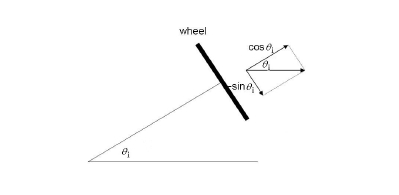
\includegraphics[scale=1.1]{./holonomic/linear_speed}
\caption{ Prędkość liniowa dużego koła szwedzkiego i małych kółek, gdy robot porusza się wzdłuż osi OX }\label{fig:linear_speed}
\end{figure}

\section{Obliczanie profilu prędkości liniowej robota \label{sec:trapezoid_vel}}
Znając już powiązanie pomiędzy prędkością obrotową kół a prędkością liniową i obrotową robota, ostatnim elementem jest wyznaczenie prędkości prowadzących 
robota do zadanego punktu. Należy przy tym uwzględnić takie parametry robota jak przyspieszenie i opóźnienie. W tym celu skorzystano z metody opisanej w 
\cite{trapezy1} oraz \cite{trapezy2}. Polega ona na dekompozycji dwuwymiarowego problemu sterowania robotem do dwóch problemów jednowymiarowych, tak jak to zaprezentowano
na rysunku \ref{fig:trapezoid_rule}. Ruch robota w kierunku osi OX i w kierunku osi OY jest rozpatrywany osobno. 
\begin{figure}[H]
\centering
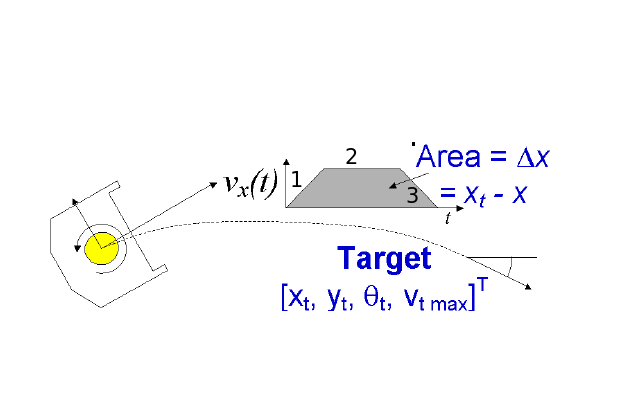
\includegraphics[scale=0.7]{./holonomic/trapezoid_rule}
\caption{ Dekompozycja sterowania robotem w 2D na dwa niezależne zadania w 1D }\label{fig:trapezoid_rule}
\end{figure}
Podejście to jest znane w robotyce pod nazwą trapezoidalnego profilu prędkości.
Zakłada ono, że robot powinien starać się osiągnąć swoją maksymalną prędkość poruszając się ze stałym przyspieszeniem (sytuacja zaznaczona numerem $1$ na rysunku).
Następnie powinien poruszać się ze stałą prędkością, aż do momentu kiedy tuż przed punktem docelowym zaczyna hamować (sytuacje $2$ i $3$ na rysunku). 
W szczególnym przypadku profil prędkości może przybrać formę trójkąta.
Prędkość obliczana jest według następujących reguł:
\begin{enumerate}
\item Jeśli bieżąca prędkość spowoduje oddalenie się robota od celu to wyhamuj do 0.
\item Jeśli robot poruszając się z bieżąca prędkością przejedzie cel to także należy zatrzymać go.
\item Gdy bieżąca prędkość przekracza maksymalną, wyhamuj do prędkości maksymalnej.
\item Oblicz trójkątny profil prędkości prowadzącej do celu.
\item Jeśli w obliczonym rozkładzie prędkość przekracza w jakimkolwiek momencie maksimum to należy obliczyć trapezoidalny profil. 
\end{enumerate} 

\section{Dryblowanie z piłką}
We wcześniejszym podrozdziale rozwiązano problem sterowania omnikierunkową bazą jezdną. Osobnym zadaniem jest wyznaczanie prędkości robota w sytuacji kiedy posiada on piłkę.
Robot dryblujący z piłką nie może poruszać się z pełną dowolnością, tak aby nie stracić nad nią kontroli. Problem ten został dokładnie zaprezentowany w \cite{dribbling}. W publikacji co prawda skupiono
się na modelu robota z rozgrywek \emph{Middle-size League}, jednak zaprezentowany algorytm znajduje zastosowanie także w lidze małych robotów.
Na rysunku \ref{fig:omni_base_dribbling} przedstawiono bazę jezdną z zaznaczonym globalnym układem współrzędnych $[X_w;Y_w]$ oraz związanym ze sterowanym robotem $[X_m;Y_m]$. Za pomocą wektora $v_r$ zaznaczono
prędkość liniową z jaką porusza się robot.
\begin{figure}[h]
\centering
\includegraphics[scale=0.5]{./holonomic/omni_base_dribbling}
\caption{Omnikierunkowa baza jezdna stosowana w rozgrywkach średnich robotów. Źródło \cite{dribbling}}\label{fig:omni_base_dribbling}
\end{figure}
Natomiast na rysunku \ref{fig:dribbling_ball} przedstawiona została sytuacja gdy robot jest w~posiadaniu piłki. Krzywa $P$ oznacza trajektorię, po której porusza się zawodnik. Aby nie stracić piłki,
punkt $E$ znajdujący się dokładnie na wprost robota w odległości $L$ równej promieniowi piłki, powinien pokrywać się z jej środkiem. Zadaniem algorytmu sterującego dryblującym robotem, jest zatem wyznaczenie
prędkości obrotowej, takiej aby środek piłki znajdował się w otoczeniu punkt $E$. W przypadku robotów z ligi \emph{Small-size League} $L=r_{ball}+r_{robot} +w_{dribbler}$.
\begin{figure}[h]
\centering
\includegraphics[scale=0.5]{./holonomic/dribbling_ball}
\caption{ Pozycja piłki w układzie współrzędnych związanym z robotem. Źródło \cite{dribbling} }\label{fig:dribbling_ball}
\end{figure}
Na rysunku \ref{fig:ball_control} przedstawiono robota wykonującego obrót z piłką. W momencie kiedy robot wraz z piłką poruszają się po łuku $c$, piłka posiada pewne przyspieszenie dośrodkowe,
$a_b=cv_e$ powodujące jej odchylenie od punktu $E$. Na rysunku symbolem $\Delta\Theta$ zaznaczono odchylenie kątowe wynikające właśnie z działania siły dośrodkowej, które należy minimalizować,
 aby robot nie stracił kontroli nad piłką. Odchylenie to można zamodelować jako: $\Delta\Theta=k_{\Theta}cv_{d}^2$ , gdzie $k_{\Theta}$ jest dobranym empirycznie parametrem.
\begin{figure}[h]
\centering
\includegraphics[scale=0.5]{./holonomic/ball_control}
\caption{ Odchylenie piłki od idealnego położenia podczas manewrowania. Źródło \cite{dribbling} }\label{fig:ball_control}
\end{figure}
W przypadku idealnym rotacja robota wykonującego manewr powinna być równa: $\Theta_{d}=\Theta_{P} + \Delta\Theta$, gdzie $\Theta_{P}$ jest nachyleniem stycznej do trajektorii, po której porusza się robot w punkcie
będącym rzutem prostokątnym $E$ na ścieżkę.  Do regulacji rotacji robota posiadającego piłkę w publikacji \cite{dribbling}
wykorzystano regulator PD. Prędkość obrotowa obliczana jest zatem następująco: $\omega=k_p(\Theta_d -\Theta) +k_d(\dot{\Theta}_d -\dot{\Theta} )$. Parametry $k_p$ oraz $k_d$ są dobierane empirycznie.

